% AdjList — Embedded property storage layout
\documentclass[tikz,border=4mm]{standalone}
\usepackage[T1]{fontenc}
\usepackage{lmodern}
% Shared TikZ styles for Flexograph table-layout diagrams.
% Include with % Shared TikZ styles for Flexograph table-layout diagrams.
% Include with % Shared TikZ styles for Flexograph table-layout diagrams.
% Include with \input{schema_styles} in each standalone figure.

\usetikzlibrary{shapes.multipart, arrows.meta, positioning, fit, calc, backgrounds}

% ── Colour palette ──────────────────────────────────────────────────
\definecolor{tblheader}{HTML}{2C3E50}   % dark blue-grey header bar
\definecolor{tblbody}{HTML}{ECF0F1}     % light grey table body
\definecolor{sentbg}{HTML}{D5DBDB}      % sentinel row shading
\definecolor{cgTemporal}{HTML}{AED6F1}  % column group: temporal
\definecolor{cgName}{HTML}{A9DFBF}      % column group: name
\definecolor{cgContact}{HTML}{F9E79F}   % column group: contact
\definecolor{cgLocation}{HTML}{F5CBA7}  % column group: location
\definecolor{cgContent}{HTML}{D2B4DE}   % column group: content
\definecolor{structClr}{HTML}{85929E}   % structural table border
\definecolor{propClr}{HTML}{2980B9}     % property table border
\definecolor{secClr}{HTML}{27AE60}      % secondary table border
\definecolor{arrowClr}{HTML}{7F8C8D}    % relationship arrows

% ── Node styles ─────────────────────────────────────────────────────
\tikzset{
  % Table header bar
  tblhdr/.style={
    rectangle, draw=tblheader, fill=tblheader,
    text=white, font=\sffamily\bfseries\footnotesize,
    minimum width=#1, minimum height=5mm, inner sep=2pt,
    align=center,
  },
  tblhdr/.default=38mm,
  % Table body (single cell / row)
  tblcell/.style={
    rectangle, draw=tblheader!40, fill=tblbody,
    font=\sffamily\scriptsize, minimum width=#1,
    minimum height=4.5mm, inner sep=2pt, align=center,
  },
  tblcell/.default=38mm,
  % Sentinel-row variant
  sentcell/.style={
    tblcell=#1, fill=sentbg,
  },
  sentcell/.default=38mm,
  % Column-group cell (coloured)
  cgcell/.style 2 args={
    tblcell=#1, fill=#2,
  },
  % Key column (narrower, left-aligned)
  keycell/.style={
    tblcell=#1, font=\sffamily\scriptsize\itshape,
  },
  keycell/.default=18mm,
  % Format annotation
  fmtlabel/.style={
    font=\sffamily\tiny\color{tblheader!70}, anchor=north west,
  },
  % Dashed grouping box
  groupbox/.style={
    rectangle, rounded corners=2pt, draw=#1, densely dashed,
    line width=0.6pt, inner sep=3pt,
  },
  groupbox/.default=structClr,
  % Relationship arrow
  relarrow/.style={
    -{Stealth[length=2.5mm]}, arrowClr, line width=0.5pt,
  },
  % Label for relationship
  rellabel/.style={
    font=\sffamily\tiny\color{arrowClr}, midway, fill=white, inner sep=1pt,
  },
}
 in each standalone figure.

\usetikzlibrary{shapes.multipart, arrows.meta, positioning, fit, calc, backgrounds}

% ── Colour palette ──────────────────────────────────────────────────
\definecolor{tblheader}{HTML}{2C3E50}   % dark blue-grey header bar
\definecolor{tblbody}{HTML}{ECF0F1}     % light grey table body
\definecolor{sentbg}{HTML}{D5DBDB}      % sentinel row shading
\definecolor{cgTemporal}{HTML}{AED6F1}  % column group: temporal
\definecolor{cgName}{HTML}{A9DFBF}      % column group: name
\definecolor{cgContact}{HTML}{F9E79F}   % column group: contact
\definecolor{cgLocation}{HTML}{F5CBA7}  % column group: location
\definecolor{cgContent}{HTML}{D2B4DE}   % column group: content
\definecolor{structClr}{HTML}{85929E}   % structural table border
\definecolor{propClr}{HTML}{2980B9}     % property table border
\definecolor{secClr}{HTML}{27AE60}      % secondary table border
\definecolor{arrowClr}{HTML}{7F8C8D}    % relationship arrows

% ── Node styles ─────────────────────────────────────────────────────
\tikzset{
  % Table header bar
  tblhdr/.style={
    rectangle, draw=tblheader, fill=tblheader,
    text=white, font=\sffamily\bfseries\footnotesize,
    minimum width=#1, minimum height=5mm, inner sep=2pt,
    align=center,
  },
  tblhdr/.default=38mm,
  % Table body (single cell / row)
  tblcell/.style={
    rectangle, draw=tblheader!40, fill=tblbody,
    font=\sffamily\scriptsize, minimum width=#1,
    minimum height=4.5mm, inner sep=2pt, align=center,
  },
  tblcell/.default=38mm,
  % Sentinel-row variant
  sentcell/.style={
    tblcell=#1, fill=sentbg,
  },
  sentcell/.default=38mm,
  % Column-group cell (coloured)
  cgcell/.style 2 args={
    tblcell=#1, fill=#2,
  },
  % Key column (narrower, left-aligned)
  keycell/.style={
    tblcell=#1, font=\sffamily\scriptsize\itshape,
  },
  keycell/.default=18mm,
  % Format annotation
  fmtlabel/.style={
    font=\sffamily\tiny\color{tblheader!70}, anchor=north west,
  },
  % Dashed grouping box
  groupbox/.style={
    rectangle, rounded corners=2pt, draw=#1, densely dashed,
    line width=0.6pt, inner sep=3pt,
  },
  groupbox/.default=structClr,
  % Relationship arrow
  relarrow/.style={
    -{Stealth[length=2.5mm]}, arrowClr, line width=0.5pt,
  },
  % Label for relationship
  rellabel/.style={
    font=\sffamily\tiny\color{arrowClr}, midway, fill=white, inner sep=1pt,
  },
}
 in each standalone figure.

\usetikzlibrary{shapes.multipart, arrows.meta, positioning, fit, calc, backgrounds}

% ── Colour palette ──────────────────────────────────────────────────
\definecolor{tblheader}{HTML}{2C3E50}   % dark blue-grey header bar
\definecolor{tblbody}{HTML}{ECF0F1}     % light grey table body
\definecolor{sentbg}{HTML}{D5DBDB}      % sentinel row shading
\definecolor{cgTemporal}{HTML}{AED6F1}  % column group: temporal
\definecolor{cgName}{HTML}{A9DFBF}      % column group: name
\definecolor{cgContact}{HTML}{F9E79F}   % column group: contact
\definecolor{cgLocation}{HTML}{F5CBA7}  % column group: location
\definecolor{cgContent}{HTML}{D2B4DE}   % column group: content
\definecolor{structClr}{HTML}{85929E}   % structural table border
\definecolor{propClr}{HTML}{2980B9}     % property table border
\definecolor{secClr}{HTML}{27AE60}      % secondary table border
\definecolor{arrowClr}{HTML}{7F8C8D}    % relationship arrows

% ── Node styles ─────────────────────────────────────────────────────
\tikzset{
  % Table header bar
  tblhdr/.style={
    rectangle, draw=tblheader, fill=tblheader,
    text=white, font=\sffamily\bfseries\footnotesize,
    minimum width=#1, minimum height=5mm, inner sep=2pt,
    align=center,
  },
  tblhdr/.default=38mm,
  % Table body (single cell / row)
  tblcell/.style={
    rectangle, draw=tblheader!40, fill=tblbody,
    font=\sffamily\scriptsize, minimum width=#1,
    minimum height=4.5mm, inner sep=2pt, align=center,
  },
  tblcell/.default=38mm,
  % Sentinel-row variant
  sentcell/.style={
    tblcell=#1, fill=sentbg,
  },
  sentcell/.default=38mm,
  % Column-group cell (coloured)
  cgcell/.style 2 args={
    tblcell=#1, fill=#2,
  },
  % Key column (narrower, left-aligned)
  keycell/.style={
    tblcell=#1, font=\sffamily\scriptsize\itshape,
  },
  keycell/.default=18mm,
  % Format annotation
  fmtlabel/.style={
    font=\sffamily\tiny\color{tblheader!70}, anchor=north west,
  },
  % Dashed grouping box
  groupbox/.style={
    rectangle, rounded corners=2pt, draw=#1, densely dashed,
    line width=0.6pt, inner sep=3pt,
  },
  groupbox/.default=structClr,
  % Relationship arrow
  relarrow/.style={
    -{Stealth[length=2.5mm]}, arrowClr, line width=0.5pt,
  },
  % Label for relationship
  rellabel/.style={
    font=\sffamily\tiny\color{arrowClr}, midway, fill=white, inner sep=1pt,
  },
}


\begin{document}
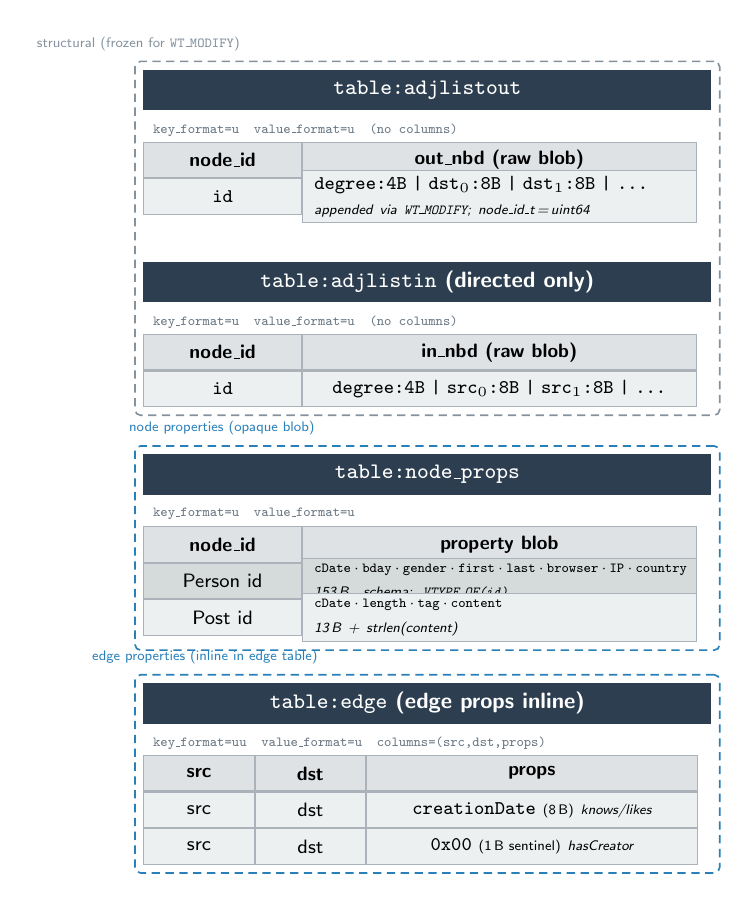
\begin{tikzpicture}[node distance=0mm]

% ════════════════════════════════════════════════════════════════════
%  TABLE: adjlistout
% ════════════════════════════════════════════════════════════════════
\node[tblhdr=72mm] (aout-hdr) {\texttt{table:adjlistout}};
\node[fmtlabel, below right=0.5mm and 0mm of aout-hdr.south west]
  {\texttt{key\_format=u\ \ value\_format=u\ \ (no columns)}};

\node[tblcell=20mm, below=4mm of aout-hdr.south west, anchor=north west,
      fill=tblheader!15, font=\sffamily\scriptsize\bfseries] (ao-ch-k) {node\_id};
\node[tblcell=50mm, right=0mm of ao-ch-k,
      fill=tblheader!15, font=\sffamily\scriptsize\bfseries] (ao-ch-v)
  {out\_nbd (raw blob)};

\node[tblcell=20mm, below=0mm of ao-ch-k] (ao-r1-k) {\texttt{id}};
\node[tblcell=50mm, right=0mm of ao-r1-k, align=left, text width=47mm] (ao-r1-v)
  {\texttt{degree:4B\;|\;dst$_0$:8B\;|\;dst$_1$:8B\;|\;\ldots}\\[0.3mm]
   {\tiny\itshape appended via \texttt{WT\_MODIFY}; node\_id\_t\,=\,uint64}};

% ════════════════════════════════════════════════════════════════════
%  TABLE: adjlistin
% ════════════════════════════════════════════════════════════════════
\node[tblhdr=72mm, below=6mm of ao-r1-k.south west, anchor=north west]
  (ain-hdr) {\texttt{table:adjlistin} {\footnotesize(directed only)}};
\node[fmtlabel, below right=0.5mm and 0mm of ain-hdr.south west]
  {\texttt{key\_format=u\ \ value\_format=u\ \ (no columns)}};

\node[tblcell=20mm, below=4mm of ain-hdr.south west, anchor=north west,
      fill=tblheader!15, font=\sffamily\scriptsize\bfseries] (ai-ch-k) {node\_id};
\node[tblcell=50mm, right=0mm of ai-ch-k,
      fill=tblheader!15, font=\sffamily\scriptsize\bfseries] (ai-ch-v)
  {in\_nbd (raw blob)};

\node[tblcell=20mm, below=0mm of ai-ch-k] (ai-r1-k) {\texttt{id}};
\node[tblcell=50mm, right=0mm of ai-r1-k] (ai-r1-v)
  {\texttt{degree:4B\;|\;src$_0$:8B\;|\;src$_1$:8B\;|\;\ldots}};

% ════════════════════════════════════════════════════════════════════
%  TABLE: node_props  (opaque blob, schema dispatched by VTYPE_OF)
% ════════════════════════════════════════════════════════════════════
\node[tblhdr=72mm, below=6mm of ai-r1-k.south west, anchor=north west]
  (np-hdr) {\texttt{table:node\_props}};
\node[fmtlabel, below right=0.5mm and 0mm of np-hdr.south west]
  {\texttt{key\_format=u\ \ value\_format=u}};

\node[tblcell=20mm, below=4mm of np-hdr.south west, anchor=north west,
      fill=tblheader!15, font=\sffamily\scriptsize\bfseries] (np-ch-k)
  {node\_id};
\node[tblcell=50mm, right=0mm of np-ch-k,
      fill=tblheader!15, font=\sffamily\scriptsize\bfseries] (np-ch-v)
  {property blob};

% Person row
\node[sentcell=20mm, below=0mm of np-ch-k] (np-r1-k) {Person id};
\node[sentcell=50mm, right=0mm of np-r1-k, align=left, text width=47mm]
  (np-r1-v) {%
  {\tiny\texttt{cDate\,$\cdot$\,bday\,$\cdot$\,gender\,$\cdot$\,first\,$\cdot$\,last\,$\cdot$\,browser\,$\cdot$\,IP\,$\cdot$\,country}}\\[0.3mm]
  {\tiny\itshape 153\,B\quad schema: \texttt{VTYPE\_OF(id)}}};

% Post row
\node[tblcell=20mm, below=0mm of np-r1-k] (np-r2-k) {Post id};
\node[tblcell=50mm, right=0mm of np-r2-k, align=left, text width=47mm]
  (np-r2-v) {%
  {\tiny\texttt{cDate\,$\cdot$\,length\,$\cdot$\,tag\,$\cdot$\,content}}\\[0.3mm]
  {\tiny\itshape 13\,B + strlen(content)}};

% ════════════════════════════════════════════════════════════════════
%  Edge props: inline in the edge table
% ════════════════════════════════════════════════════════════════════
\node[tblhdr=72mm, below=6mm of np-r2-k.south west, anchor=north west]
  (et-hdr) {\texttt{table:edge} {\footnotesize(edge props inline)}};
\node[fmtlabel, below right=0.5mm and 0mm of et-hdr.south west]
  {\texttt{key\_format=uu\ \ value\_format=u\ \ columns=(src,dst,props)}};

\node[tblcell=14mm, below=4mm of et-hdr.south west, anchor=north west,
      fill=tblheader!15, font=\sffamily\scriptsize\bfseries] (et-ch-s) {src};
\node[tblcell=14mm, right=0mm of et-ch-s,
      fill=tblheader!15, font=\sffamily\scriptsize\bfseries] (et-ch-d) {dst};
\node[tblcell=42mm, right=0mm of et-ch-d,
      fill=tblheader!15, font=\sffamily\scriptsize\bfseries] (et-ch-v) {props};

\node[tblcell=14mm, below=0mm of et-ch-s] (et-r1-s) {src};
\node[tblcell=14mm, right=0mm of et-r1-s] (et-r1-d) {dst};
\node[tblcell=42mm, right=0mm of et-r1-d] (et-r1-v)
  {\texttt{creationDate} {\tiny(8\,B)} {\tiny\itshape knows/likes}};

\node[tblcell=14mm, below=0mm of et-r1-s] (et-r2-s) {src};
\node[tblcell=14mm, right=0mm of et-r2-s] (et-r2-d) {dst};
\node[tblcell=42mm, right=0mm of et-r2-d] (et-r2-v)
  {\texttt{0x00} {\tiny(1\,B sentinel)} {\tiny\itshape hasCreator}};

% ── Grouping boxes ──────────────────────────────────────────────
\begin{pgfonlayer}{background}
  \node[groupbox=structClr, fit=(aout-hdr)(ai-r1-v),
        label={[font=\sffamily\tiny,
        text=structClr]above left:structural (frozen for \texttt{WT\_MODIFY})}] {};
  \node[groupbox=propClr, fit=(np-hdr)(np-r2-v),
        label={[font=\sffamily\tiny,
        text=propClr]above left:node properties (opaque blob)}] {};
  \node[groupbox=propClr, fit=(et-hdr)(et-r2-v),
        label={[font=\sffamily\tiny,
        text=propClr]above left:edge properties (inline in edge table)}] {};
\end{pgfonlayer}

\end{tikzpicture}
\end{document}
